\documentclass{article}
\usepackage[utf8]{inputenc}

\usepackage[a4paper, total={7in, 12in}]{geometry}


\usepackage{graphicx}
\graphicspath{ {../results/} }


\title{\textbf{Is there autocorrelation in temperature in Florida in the twentieth century?\vspace{-0.5em}}}
\author{Booming Bonobos // January 2022}
%\predate{}
%\postdate{}
\date{}

\begin{document}

\maketitle

\section{Introduction \vspace{-0.5em}}

    Florida is home to over 20 million people and is one of the most biodiverse states in the United States \cite{usda}. It is also likely to face particularly significant impacts from climate change, in part due to its low topographic relief and high inter-annual variability of precipitation. It is therefore important to understand and quantify the extent of the nature and impacts of climate change in Florida to facilitate appropriate mitigating and adaptive measures. While some historical data sets indicate increasing temperatures and decreasing precipitation \cite{irizarry2013historical}, other studies have found no such trends \cite{obeysekera2011climate}. This short study uses an annual temperature dataset from Key West in Florida for the twentieth century to examine whether temperatures of one year are significantly correlated with those of the next year across years in this given location. \vspace{-1em}

\section{Methods \vspace{-0.5em}}

Using a permutation test of autocorrelation, we assess whether the correlation between mean annual temperature and year differs significantly from what would be expected from a random dataset. Autocorrelation involves finding correlations between pairs of consecutive years to test whether the temperature in one year is correlated with the temperature in the next year. We firstly calculate the autocorrelation coefficients between pairs of years for the test data, then reshuffle the temperatures of the data 100,000 times, and recalculate the autocorrelation coefficients for this null dataset. We then assess how likely the test autocorrelation coefficients are to be drawn from this null distribution by calculating what fraction of the random null autocorrelation coefficients were greater than the observed test coefficients. We used Spearman's correlation coefficient as this tests for monotonic relationships; this tests for whether the data are ordered, rather than just linear. \vspace{-1em}

\section{Results \vspace{-0.5em}}

Temperatures autocorrelated significantly across years (observed test data autocorrelation coefficient = 0.341, permutation test P = 0.00025, Figure 1), with the test data coefficient differing signficantly from the null distribution of coefficients (Figure 2). \vspace{-0.5em}

    \begin{figure}[htbp]
    \centering
    \begin{minipage}{.5\textwidth}
        \centering
        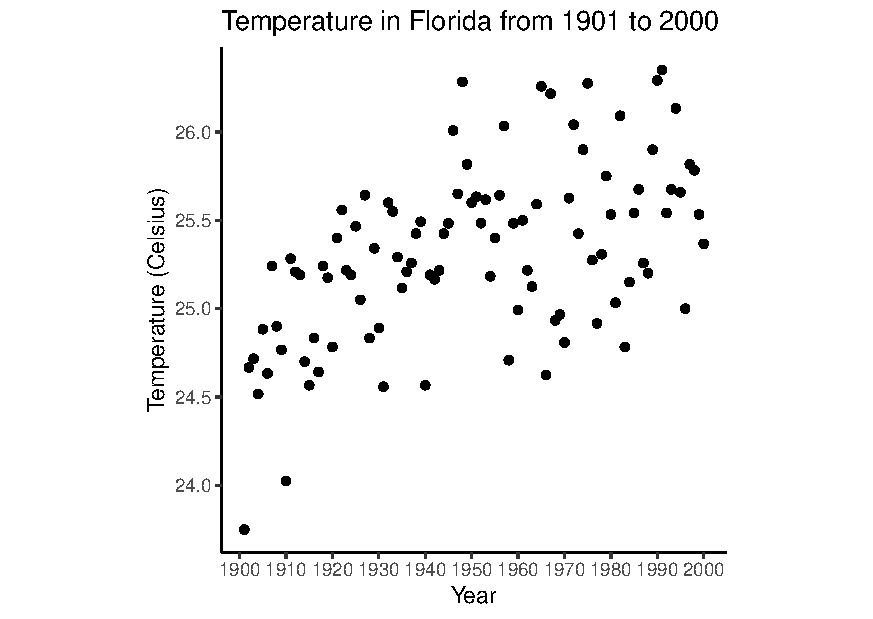
\includegraphics[scale=0.4]{DistributionFlorida.pdf}
        \caption{Annual temperature in Key West, Florida, \newline from 1901 to 2000.} 
        \label{fig.test1}
    \end{minipage}%
    \begin{minipage}{.5\textwidth}
        \centering
        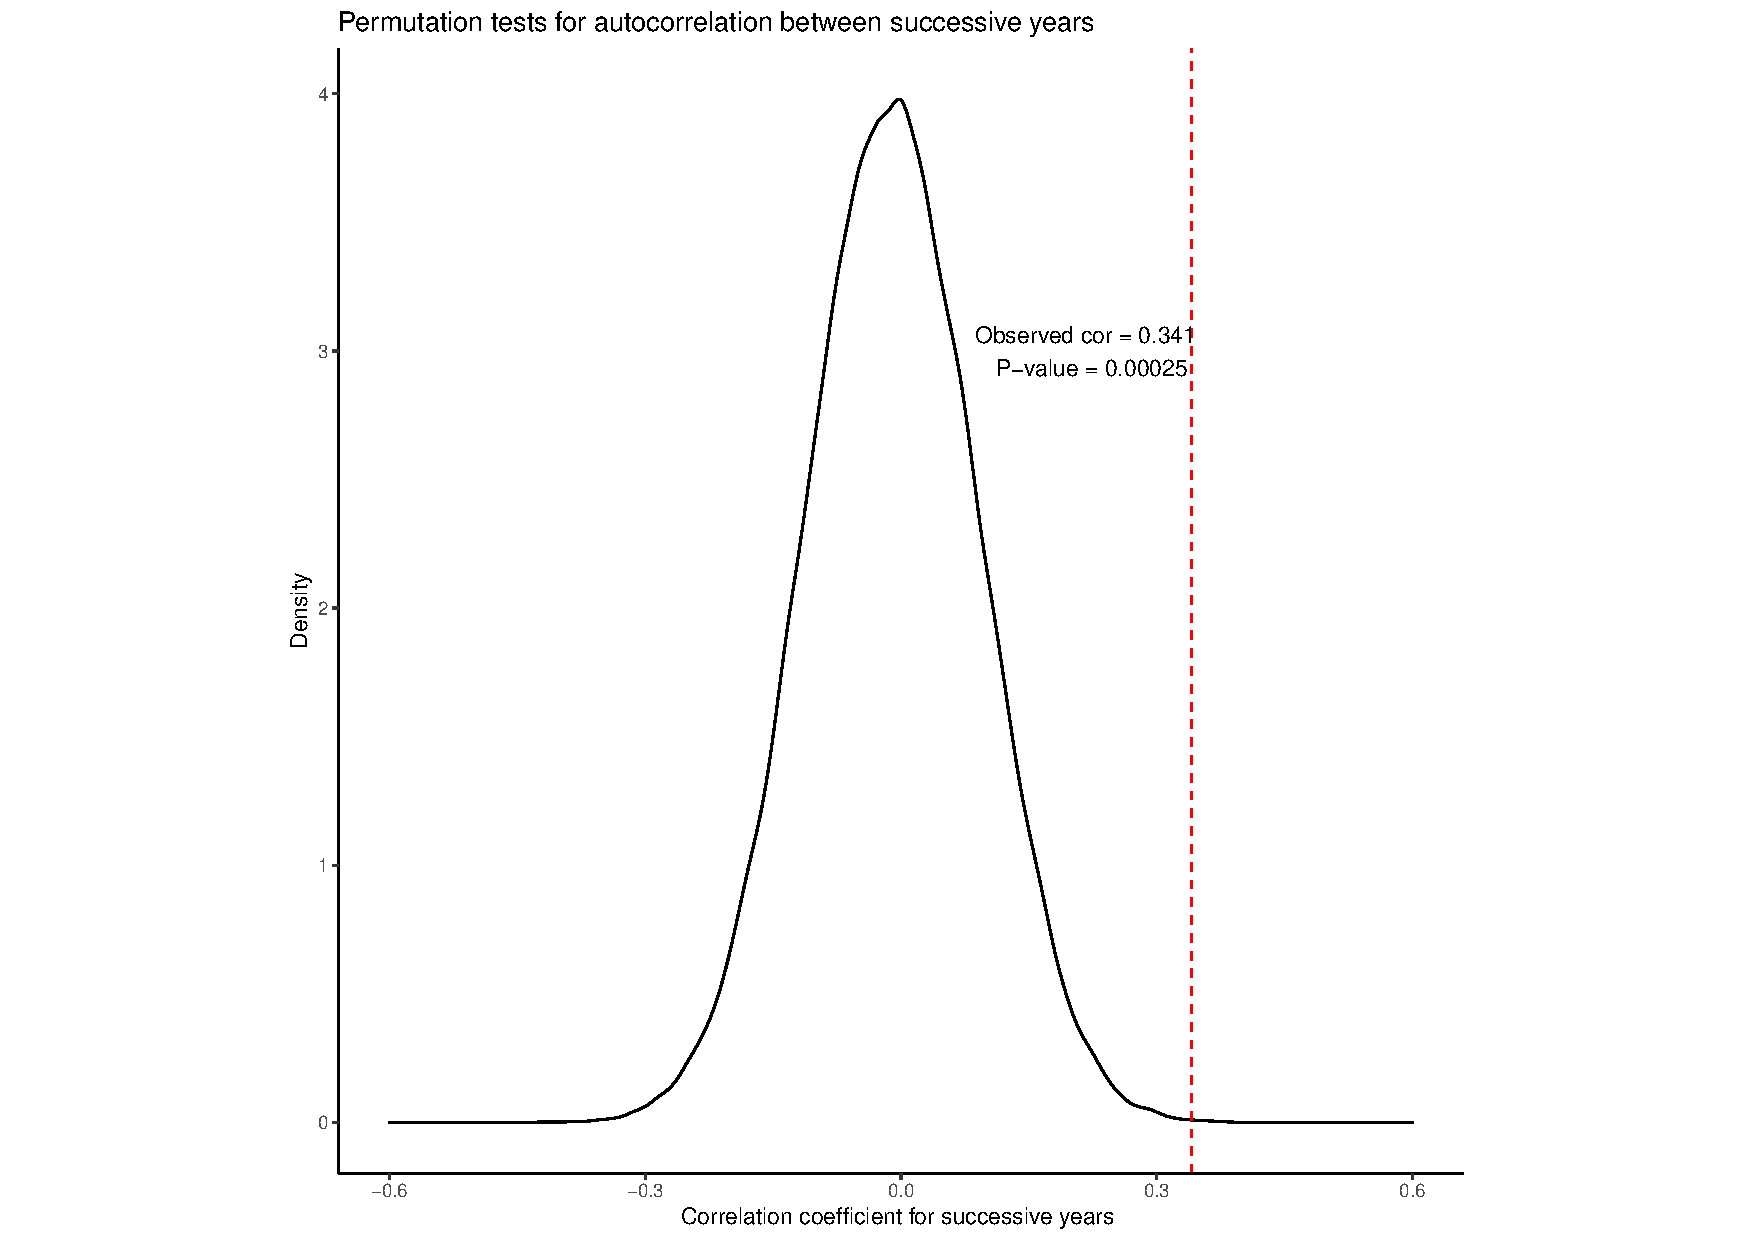
\includegraphics[scale=0.4]{PermuCorCoeff_TAutoCorr.pdf}
        \caption{Density plot of the null distribution of autocorrelation coefficients between temperatures in successive years in Key West, Florida. The blue dashed line represents the test correlation coefficient.}
        \label{fig:test2}
    \end{minipage}
    \end{figure}\vspace{-1.5em}

\section{Discussion \vspace{-0.5em}}

    This observed autcorrelation between temperatures across different years over the twentieth century in Florida suggests that changes to climate are occurring non-randomly. This result should be used to urge governments to take more action to slow climate change, to devise more adaptive measures to mitigate its negative impacts, and to combine with other data to forecast future temperature changes. With increasing availability of these long-term datasets, there is much scope for improving our ability to understand, predict, and mitigate climate change. \vspace{-1em}

\bibliographystyle{plain}
	
	\bibliography{Floridabiblio}


\end{document}
